% Source p.2 (966). Tangency is preserved by a layout construction, not solution data.
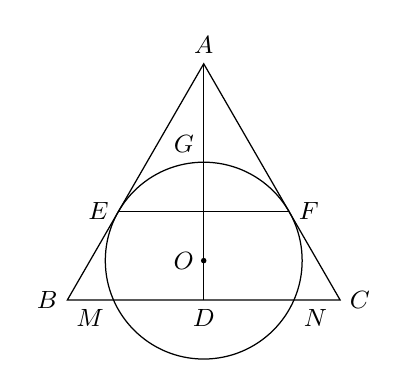
\begin{tikzpicture}[line width=.45pt,font=\small]
  \coordinate (A) at (0,3); \coordinate (B) at (-1.732,0);
  \coordinate (C) at (1.732,0); \coordinate (D) at (0,0);
  \coordinate (O) at (0,.5); \coordinate (G) at (0,1.75);
  \coordinate (E) at (-1.0825,1.125); \coordinate (F) at (1.0825,1.125);
  \coordinate (M) at (-1.1456,0); \coordinate (N) at (1.1456,0);
  \draw (A)--(B)--(C)--cycle;
  \draw (A)--(D) (E)--(F);
  \draw (O) circle (1.25);
  \fill (O) circle (1pt);
  \node[above] at (A) {$A$}; \node[left] at (B) {$B$};
  \node[right] at (C) {$C$}; \node[below] at (D) {$D$};
  \node[left] at (O) {$O$}; \node[above left] at (G) {$G$};
  \node[left] at (E) {$E$}; \node[right] at (F) {$F$};
  \node[below left] at (M) {$M$}; \node[below right] at (N) {$N$};
\end{tikzpicture}
